\section*{\large 問題2}
\ 
ファン圧力比$\pi_f$を求める式は、
\begin{equation}
 \pi_f = \left\{\frac{c_{pt}(T_{t4}-T_j)\lambda_{op} \eta}{c_{pc}T_{t1}\mu}+1\right\}^{\frac{\kappa_c}{\kappa_c-1}}
\end{equation}
となる。これより得たファン圧力比$\pi_f$の値を以下に示す。
\begin{table}[htb]
 \begin{center}
  \caption{各バイパス比におけるファン圧力比}
  \begin{tabular}{|l|r|} \hline
    バイパス比$\mu [-]$  &  最適 ファン圧力比  $\pi_f [-]$ \\  \hline
                      0  &   -                             \\  \hline
                      1  &   1.804124844                   \\  \hline
                      2  &   1.526961406                   \\  \hline
                      6  &   1.219912007                   \\  \hline
                      10 &   1.138721282                   \\  \hline
                      15 &   1.094885139                   \\  \hline
                      20 &   1.072093843                   \\  \hline
   
  \end{tabular}
 \end{center}
\end{table}

\begin{figure}[t]
 \begin{center}
  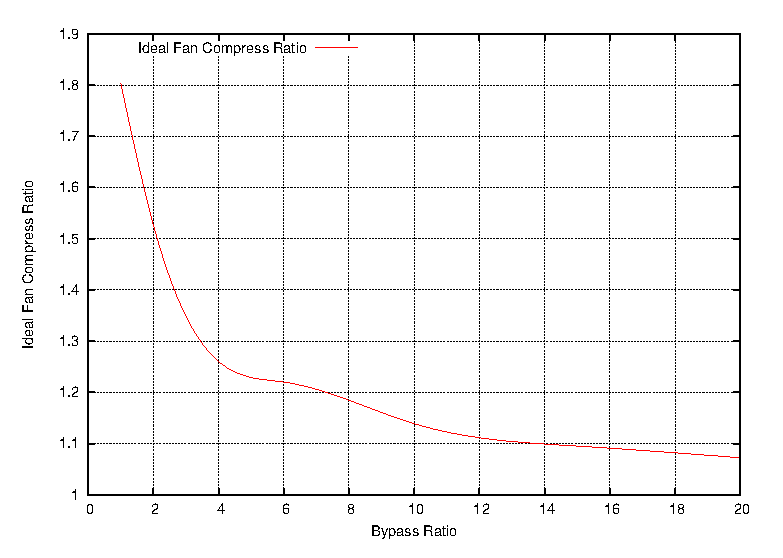
\includegraphics[width=10.0cm]{eps/body2_1.eps}
  \caption{バイパス比との関係}
 \end{center}
\end{figure}
